\section{Insights into DL Benchmark Workflows}
\label{sec:workflow-main}

As we are trying to benchmark various aspects of the applications and
the systems utilizing Deepl Learning, we need to be able to easily
formulate runtime variables that thake into account different control
parameters either of the algorithm or the underlaying system and
hardware.

Furthermore it is beneficial to be able to coordinate benchmarks on
remote machines either on a single system or while using multiple
system in conjunction as hybrid and heterogeneous multi HPC
systems. These concepts are similar to thos found in cloud and Grid
computing for job services \citep{las-infogram} and for workflows
\citep{las-workflow,las07-workflow}. However, the focus here is on
that the services provided are controled by the application user and
not necessarily by the cloud or HPC provider. THus we distigush the
need for a workflow service that can utilize heterogeneous HPC systems
while leveraging the same parameter set to conduct a benchmark for
comparision. Such a framework was presented by von Laszewski,
Fleisher, et.al. in \citep{las-22-arxiv-workflow-cc}.

In addition, we need a mechanism to create various runs with different
parameters. One of the issues we run into is that often our runtime
needs exceed that of a single job submission and although job arrays
and custom configurations while allowing longer scheduling times could
be applied, they are typically not implemented in an educational
setting. Thus it is often more convenient to create jobs that fall
within the limits of the HPC centers policies and split the
benchmarking tasks across a number of jobs, based on the parameter
permutations.

For this reason von Laszewski, Knuuti at.al. have implemented
cloudmesh-sbatch that provides a batch job generator creating a over a
permutation of experiment parameters that are defined in a
configuration file. The tool will create for each job its own
subdirectory, copy the code and configuration files into it and create
a shell script that lists all jobs to be submitted to the queuing
system.

Furthermore we need a simple system to measure the performance and
energy, while communicationg the data in an easy fashion to the
users. THis system was developed by von Laszewski and contains two
components (a) a general stopwatch  (b) a mechanism to monitor the GPU as discussed in \label{sec:monitoring}.

We describe these systems briefly while focussing on the applicability
for benchmarks.

\subsection{Cloudmesh Monitoring}
\label{sec:monitoring}

To conduct monitoring of time we have provided for years a conveneient
StopWatch package in Python \cite{cloudmesh-stopwatch}.  It is very
easy to use and is focused on runtime execution monitoring of time
consuming portions in a single threaded Python application. Althouh
MLCommons provides their own time measuring component, called mllog,
it is clear form the name that the focus is to create entries in a log
file that may not easily readable by a human and may require
postprocessing to make usable. In contrast our library contans not
only simple labeled \vreb|start| and \verb|stop| methods, It also
provides a convenient mechanism to print human readbale customizable
performance tables. This is especially important during a debugging
phase when benchmarks are developed. Morover we also have developw a
plugin interface to mllog, that allows us to automatically create
mllog entries into an additonal log file, so the data may be used
within MLCommons through specialized anlaytics programs also. A simple
use case is depicted next

\begin{verbatim}
    from cloudmesh.common import StopWatch 
    Stopwatch.start("earthquake")
    ... run the earthqake code ...
    Stopwatch.stop("earthquake")
    Stopwatch.benchmark() # prints the current results
\end{verbatim}

In addition to the StopWatch we have developed a simple commandline
tool that can be used for example in batch scripts to monitor the GPU
performance characteristics such as energy, temperature and other
arameters \cite{cloudmesh-gpu}. The tool can be started in a batch
script as follwos and is currently supporting NVIDIA GPUs

\begin{verbatim}
    cms gpu watch --gpu=0 --delay=0.5 --dense > gpu0.log &
\end{verbatim}


Monitoring time and system GPU information can provide significant
insights into the applications performance characteristics. It is
significant for planing a time effective scedule for parameters while
running a subset of planed experiments.


\subsection{Cloudmesh-sbatch}
\label{sec:workflow-sbatch}


We describe cloudmesh-sbatch

\subsection{Cloudmesh-cc}
\label{sec:workflow-cc}

todo \citep{las-22-arxiv-workflow-cc}

\begin{itemize}
\item Different graphics cards

\item Different epochs of training

\item Create workflow for cloudmask
\end{itemize}


\subsubsection{Analytics Service Pipelines}

In many cases, a big data analysis is split up into multiple
subtasks. These subtasks may be reusable in other analytics
pipelines. Hence it is desirable to be able to specify and use them in
a coordinated fashion allowing the reuse of the logic represented by
the analysis. Users must have a clear understanding of what the
analysis is doing and how it can be invoked and integrated.

The analysis must include a clear and easy-to-understand specification
that encourages reuse and provides sufficient details about its
functionality, data dependency, and performance. Analytics services
may have authentication, autorotation, and access controls built in
that enable access by users controlled by the service providers.



\begin{figure}[htb]
\centering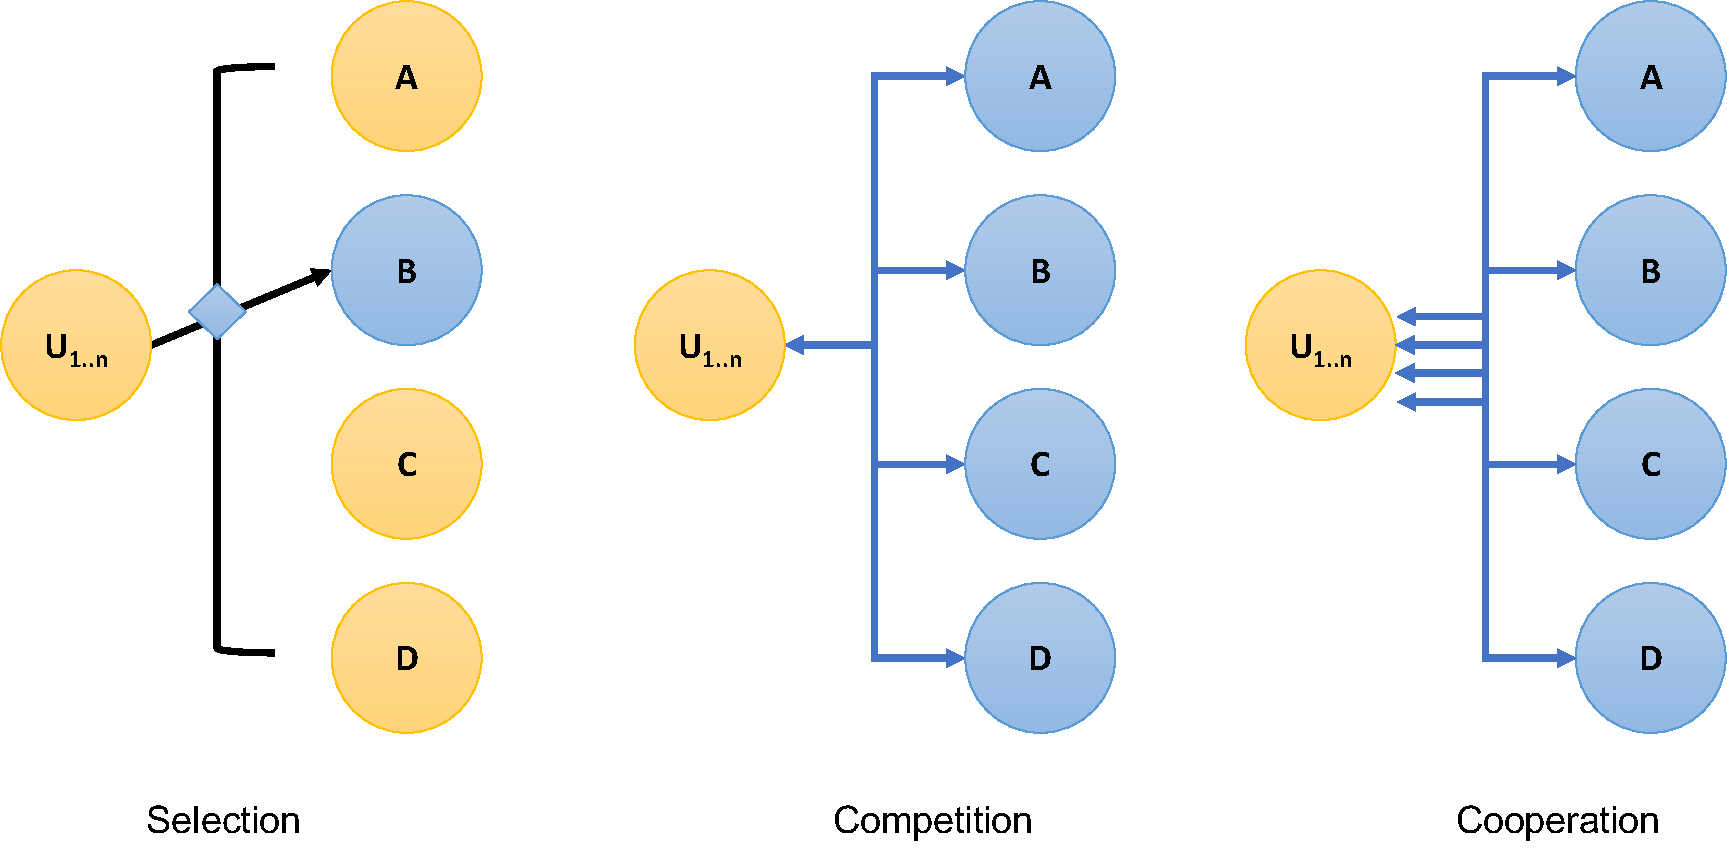
\includegraphics[width=0.75\columnwidth]{images/processes-nist.pdf}
\label{fig:service-interaction}
\caption{Service Interaction.}
\end{figure}


\subsubsection{Workflow Compute Coordinator}

High-performance computing (HPC) is for decades a very important tool
for science. Scientific tasks can be leveraging the processing power
of a supercomputer so they can run at previously unobtainable high
speeds or utilize specialized hardware for acceleration that otherwise
are not available to the user. HPC can be used for analytic programs
that leverage machine learning applied to large data sets to, for
example, predict future values or to model current states. For such
high-complexity projects, there are often multiple complex programs
that may be running repeatedly in either competition or cooperation.
This may include resources in the same or different data centers. We
developed a hybrid multi-cloud analytics service framework that was
created to manage heterogeneous and remote workflows, queues, and
jobs.  It can be used through a Python API, the command line, and a
REST service. It is supported on multiple operating systems like
macOS, Linux, and Windows 10 and 11.  The workflow is specified via an
easy-to-define YAML file.  Specifically, we have developed a library
called Cloudmesh Compute Coordinator (cloudmesh-cc) that adds workflow
features to control the execution of jobs on remote compute resources,
while at the same time leveraging capabilities provided by the local
compute environments to direct interface with graphical
visualizations better suited for the desktop. The goal is to provide
numerous workflows that in cooperation enhance the experience of the
analytics tasks. This includes a REST service and command line tools
to interact with it.


\begin{figure}[htb]
\centering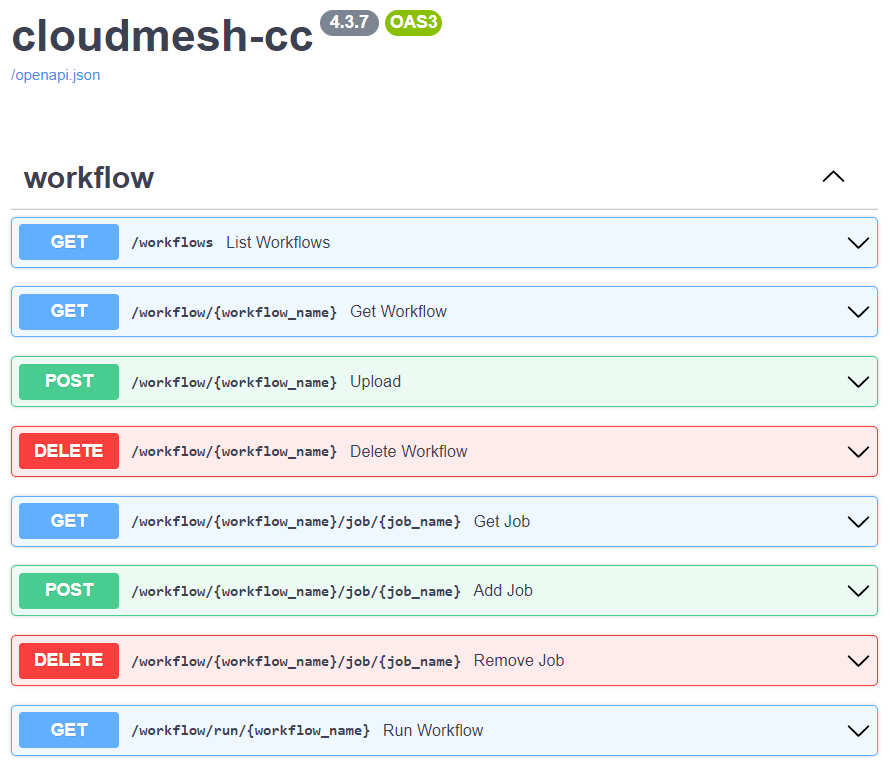
\includegraphics[width=0.7\columnwidth]{images/fastapi-service.png}
\caption{Fast API Workflow Service.}
% better resolution
\label{fig:fastapi-cc}
\end{figure}

\begin{figure}[htb]
    \centering
    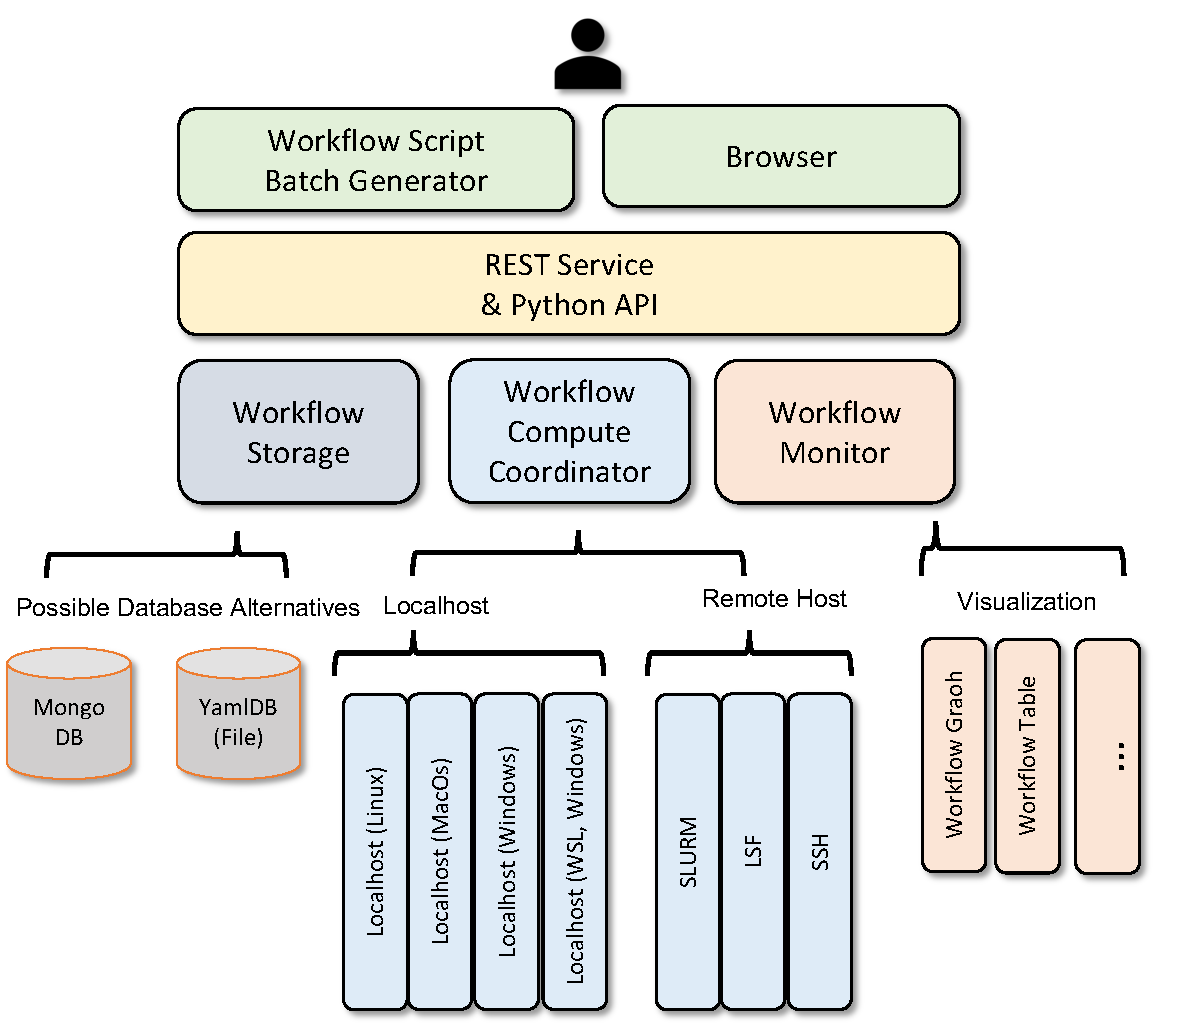
\includegraphics[width=0.50\columnwidth]{images/cloudmesh-cc-new.pdf}
    \caption{Architecture Workflow Service.}
    \label{fig:cc-2}
\end{figure}

\begin{figure}[htb]
    \centering
    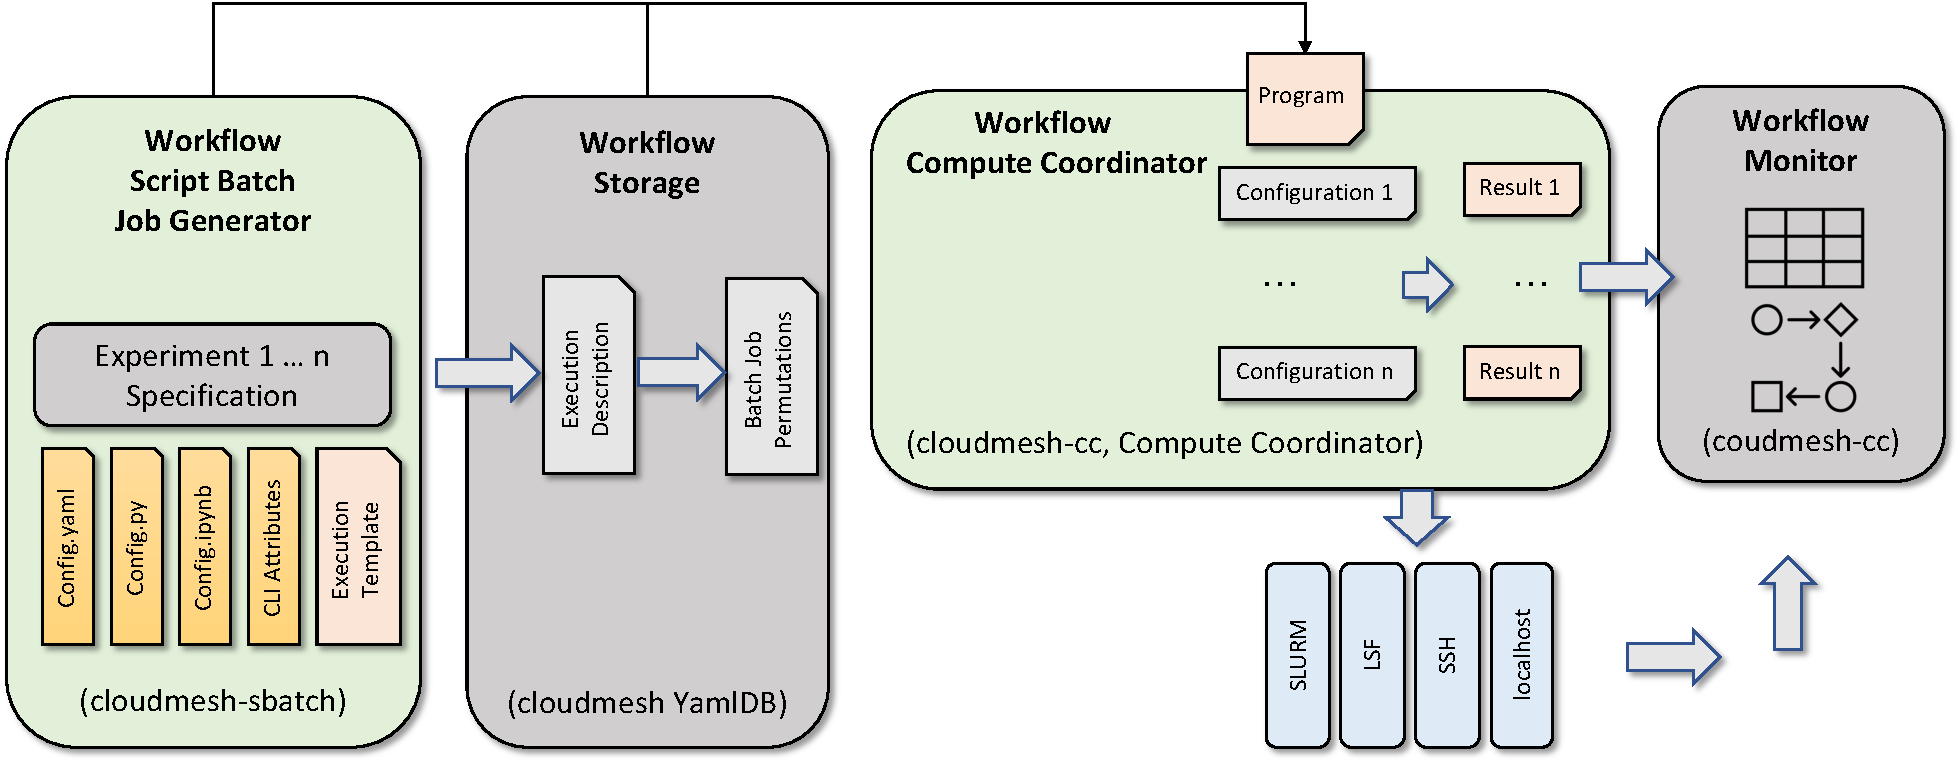
\includegraphics[width=0.70\columnwidth]{images/cloudmesh-sbatch-new.pdf}
    \caption{Workflow Script Batch Generator.}
    \label{fig:cm-sbatch}
\end{figure}

\begin{figure}[htb]
    \centering
    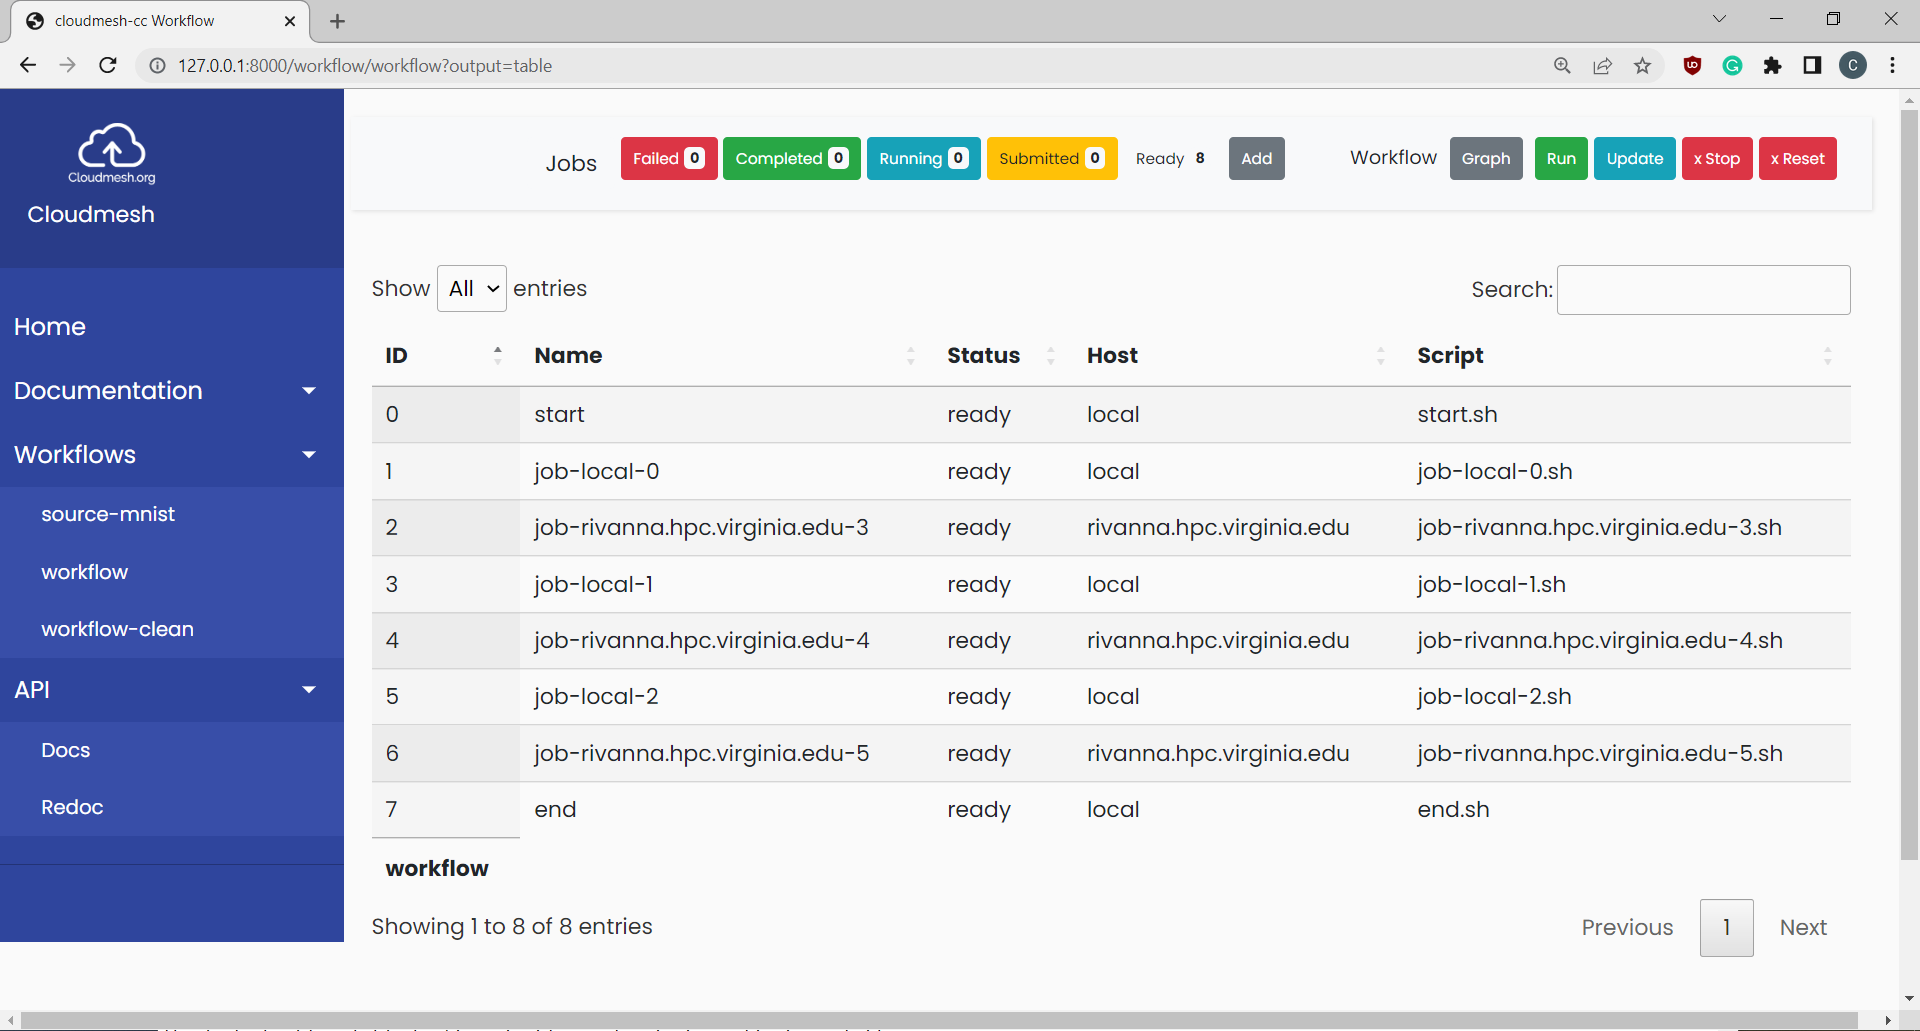
\includegraphics[width=0.70\columnwidth]{images/cc-1.png}
    \caption{Workflow user interface. }
    \label{fig:cc-3}
\end{figure}


We have tested the framework while running various MNIST application
examples, including include Multilayer Perceptron, LSTM (Long
short-term memory), Auto-Encoder, Convolutional, and Recurrent Neural
Networks, Distributed Training, and PyTorch training.  A much lager
application using earthquake prediction has also been used.

Figure \ref{fig:fastapi-cc} shows the REST specification and
\ref{fig:cc-2} shows the architecture.
